\documentclass[a4paper, 10pt]{article}
\usepackage[margin=0.5in]{geometry}

\usepackage{blindtext}
\usepackage{multicol}
\usepackage{booktabs}
\usepackage{amsmath}
\usepackage{mathtools}
\usepackage{float}
\usepackage{graphicx}
\usepackage{enumitem}
\usepackage{hyperref}
\usepackage{comment}

\graphicspath{ {../outputs/}{../data/} }


\setlength{\columnsep}{1cm}
\title{ENPM 673: Perception for Autonomous Robots - Project 2}
\author{Aswath Muthuselvam \\ aswath@umd.edu}
\date{9th March 2022}

\begin{document}
	\maketitle
	\newlist{contract}{enumerate}{10}
	\setlist[contract]{label*=\arabic*.}
	\setlistdepth{10} 
	
	\begin{figure}[b]
		\centering
		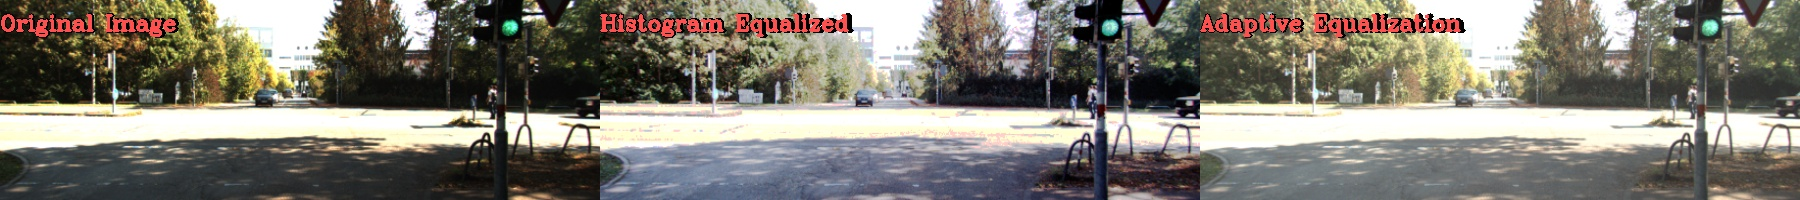
\includegraphics[width=\textwidth]{/histogram_and_adaptive.jpg}
		\caption{Original Image(left), Histogram Equalization(middle) and Adaptive Equalization(right)}
		\label{fig:HistEQ}
	\end{figure}
	
	\begin{multicols}{2}
		
		\section{Histogram equalization}
		The 24 images that was provided is taken and histogram is calculated with 256 bins, in all 3 channels-red, green and blue. Next, the cumulative distribution is calculated by summing all this bins till the current bin. This distribution is normalized and with a maximum  value of 256. A copy of this normalized value is also saved, this reduces the computation time as it can directly be applied to the subsequent $N$ video as they will have similar color distribution. The Adaptive equalization perform Gamma correction on the given image. The gamma correction of input pixel to output image is shown in Equation \ref{eq:gamma}. I took $\gamma$ is taken as 1.5.  The comparison between Original image, Histogram Equalized image and Adaptive Equalized image is shown in Figure \ref{fig:HistEQ} in the same order.
		
		\begin{equation} \label{eq:gamma}
		I_{out}=I_{in}^{\gamma}
		\end{equation}
		
		\section{Straight Lane Detection}
		In this section, I will describe the straight line detection approach I took and my thought process as I solved the problem. The video given to us appears to be sourced from the video feed of a car's dashcam. The car is seen to be driving straight in the same lane. My first thought was to filter the out the white lane lines form the original color image. Hence, I thresholded the image in RGB color space, removing all the low intensity pixels leaves us with only the white lane lines. This video does not contain any white cars unlike the curved lane detection, the steps I took to make the car disappear will be described in the next section. To identify the sweet spot of threshold levels, I created a slider to qualitatively inspect the visibility of lane lines and the background. After obtaining a satisfied values of lower limit RGB values as $(215, 123, 119)$, and upper limit RGB values as $(255, 130, 140)$, I hardcoded these in the program, henceforth, these values will be used to obtain the lane mask image. A preview of thresholding process of curve line detection is shown in Figure \ref{fig:thresh}. 
		
		After obtaining the lane mask, I used hough lines to get the equation of lane lines. However, I found that cv2.HoughLinesP() gives line segments, which was more convenient to work with. Next, I calculate the length of the line segments to determine the longest line and assign that side of the image as road boundary. However, I faced a problem with the line segments, even the longest line is detected as multiple shorter line segments. I tried dilating the image, but now it detects 2 long line segments. There are multiple ways to resolve this, such as eliminating all the shorter line segments near the x position where the longest line is detected. But I chose to count the distribution of white pixels along the columns of the image, by summing along the columns. I discretize the x axis(along the rows) of the image into 6 bins to create a distinction between the location of left and right lane markings, this is because, the distribution of white pixels keep changing on the patterned lane, hence at repeated intervals, all the peaks will be much closer to the continuous lane marking. and I then mark the side with most number of white pixels as road boundary as shown in the graphs in Figure \ref{fig:straight}. I assign the second most highest peaks as the lane boundary, marked in green color. I also compute the vanishing point, marked in purple color. I also flip the input image to show that the type of lane boundary is detected appropriately. 
		
		\begin{figure}[H]
			\centering
			\includegraphics[width=\columnwidth]{/straight_lane_detection.png}
			\caption{Lane detection: red line markings for road boundary, right lane for green markings. }
			\label{fig:straight}
		\end{figure}
		
		\begin{figure}[H]
			\centering
			\includegraphics[width=\columnwidth]{/straight_lane_segments.png}
			\caption{Lane detection: red line markings for road boundary, right lane for green markings. Purple circle shows the vanishing point found by the intersecting lanes.}
			\label{fig:straight_segments}
		\end{figure}
		
		A video preview of the lane segment detection method is available in this \href{https://youtu.be/6CWymeqQOWk}{YouTube link}, and the lane detection method is available in this \href{https://youtu.be/fkf3r3iCl74}{YouTube link}.
		
		\section{Predict Turn}	
		In this problem, we are given a video feed of a car making a turn on a long curvy highway. This time, the road boundary is marked in yellow and the lane boundaries is marked in white color. First, I obtained the mask of the lanes form the input image. I then look for the lines to get the homography transformation to obtain the top down view. From now on, I use this transformation, which is saved in the LaneDetector class, to detect the lane's curvature. 
		
		The subsequent frames are transformed into top down view for further processing. I divide the image into two equal havles along the original image center. I obtain the skeleton of the lane markings. I then collect all (x,y) coordinates of the the bright points. I fit the points to a degree two polynomial equation. After obtaining the coefficient of equation, I sample evenly distributed x coordinates and calculate the corresponding y coordinates and plot them. Sometimes, there are overexposed road patches and shadows on the lane lines, these causes erratic behavior of the computed polynomial. Hence, I use an average of the previously computed y coordinates corresponding to the sampled x coordinates. 
		
		The radius of curvature is calculated according to the equation and by taking 2 adjacent points and with the derivative formula. 
		
		The left lanes are colored in red and the right lane is colored in green. The inverse Homography is computed and the points are transformed from top down view to car's dashcam view. I fill the convex polygon formed by these points in yellow and highlight the current lane in the original image. 
		
		The Homographic transformation of top down view is not completely from the top because the polynomial fitting does not fit properly, due to some singularities. Presumably due to the reason of short change in x axis, there is a lot of changes in y axis. 
		
		A video preview of the curve lane detection method is available in this \href{https://youtu.be/5v3jpyDuoz4}{YouTube link}.
		
		\begin{figure}[H]
			\centering
			\includegraphics[width=\columnwidth]{/thresholding_curvelane.png}
			\caption{Lane line and color extraction}
			\label{fig:thresh}
		\end{figure}
		
		\begin{figure}[H]
			\centering
			\includegraphics[width=\columnwidth]{/curve_lane_detection.png}
			\caption{Curve Lane detection}
			\label{fig:curve}
		\end{figure}
		
		\section{Discussion}
		The details of homography is explained in the above section.
		
		Hough lines work by rotating the lines and find the maximum peak. The equation y=mx+c is reframed into m and c by varying x and y. When a point (m,c) is found, the hough space accumulator is increased. As the resolution of the bin is increased, the identified lines will have a closer representation to the actual line. 
		
		The lane detection pipeline that I built is not robust to lane changes and the might confuse the algorithm.
		In problem 1, the algorithm has no failsafe case to handle patterned lane markings, one of the lane lines will definitely be detected as road boundary.
		
		\section{Conclusion}	
		I have built a lane detection pipeline using OpenCV. All the figures are generated using a custom ImageGrid class present in utils.py file. 
		
	\end{multicols}
	
	
	
\end{document}
